\documentclass[]{article}
\usepackage{hyperref}
\usepackage[a4paper, total={6in, 8in}]{geometry}
\usepackage{caption}
\usepackage{algpseudocodex}
\usepackage{tabularray}
\usepackage{algorithm}
\usepackage{amsmath}
\usepackage{listings}
\usepackage{graphicx}
\usepackage{setspace}
\usepackage{subfiles}
\usepackage{xcolor}
\usepackage{enumerate}
\usepackage{xepersian}
\settextfont{XB Niloofar}

\begin{document}
یک سیستم تک پردازنده از روش زمان بندی صف چند سطحی
\lr{(MFQ)}
ستفاده می کند که در آن صف سطح اول و دوم از زمان بندی چرخشی
\lr{(RR)}
به ترتیب با کوانتوم زمانی ۴ و ۸ میلی ثانیه با زمان تعویض متن ۱ میلی ثانیه و سطح سوم از روش
\lr{FCFS}
استفاده می نماید. چهار فرآیند با زمان اجرای ۱۰ و ۳ و ۷ و ۲ به ترتیب در زمان های ۰ و ۳ و ۷ و ۲۴ وارد می شوند. میانگین زمان پاسخ و
زمان انتظار برای اجرای کامل فرآیندها را محاسبه کنید.
\\
ابتدا صف‌ها را نامگذاری می‌کنیم:       \\
صف با زمانبندی RR کوانتوم تایم ۴ میلی ثانبه
$\leftarrow$
A
\\
صف با زمانبندی RR کوانتوم تایم ۸ میلی ثانبه
$\leftarrow$
B
\\
صف با زمانبندی FCFS (صف آخر)
$\leftarrow$
C
\begin{table}[H]
    \centering
    \begin{tblr}{ c r}
        \begin{tblr}{|c|c|c|}
            \hline
            زمان انفجار & زمان ورود & فرآیند \\ \hline
            10          & 0         & $P_0$  \\ \hline
            3           & 3         & $P_1$  \\ \hline
            7           & 7         & $P_2$  \\ \hline
            2           & 24        & $P_3$
            \\ \hline
        \end{tblr} &
        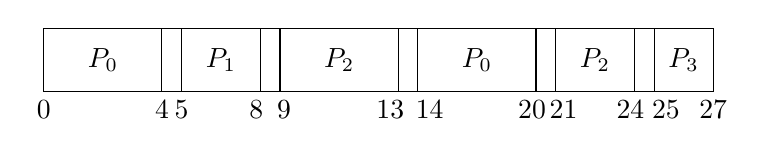
\begin{tikzpicture}
            % Draw the main rectangle
            \draw (0,0) rectangle (1.5,0.8) node[midway] {$P_0$};
            \draw (1.5,0) rectangle (1.75,0.8) node[midway] {};
            \draw (1.75,0) rectangle (2.75,0.8) node[midway] {$P_1$};
            \draw (2.75,0) rectangle (3,0.8) node[midway] {};
            \draw (3,0) rectangle (4.5,0.8) node[midway] {$P_2$};
            \draw (4.5,0) rectangle (4.75,0.8) node[midway] {};
            \draw (4.75,0) rectangle (6.25,0.8) node[midway] {$P_0$};
            \draw (6.25,0) rectangle (6.5,0.8) node[midway] {};
            \draw (6.5,0) rectangle (7.5,0.8) node[midway] {$P_2$};
            \draw (7.5,0) rectangle (7.75,0.8) node[midway] {};
            \draw (7.75,0) rectangle (8.5,0.8) node[midway] {$P_3$};


            % Draw time labels
            \node[below] at (0,0) {0};
            \node[below] at (1.5,0) {4};
            \node[below] at (1.75,0) {5};
            \node[below] at (2.7,0) {8};
            \node[below] at (3.05,0) {9};
            \node[below] at (4.4,0) {13};
            \node[below] at (4.9,0) {14};
            \node[below] at (6.2,0) {20};
            \node[below] at (6.6,0) {21};
            \node[below] at (7.45,0) {24};
            \node[below] at (7.9,0) {25};
            \node[below] at (8.5,0) {27};
        \end{tikzpicture}
    \end{tblr}
\end{table}

\begin{itemize}
    \item ابتدا در زمان صفر فقط فرآیند $P_0$ در صف A وجود دارد. پس توسط زمان بند این صف انتخاب می‌شود.
    \item حین اجرای $P_0$ فرآیند $P_1$ وارد صف A می‌شود اما آن‌را قبضه نمی‌کند.
    \item در زمان ۴ اجرای $P_0$ تمام می‌شود. این فرآیند به صف B منتقل می‌شود.
    \item در صف A فرآیند $P_1$ باقی مانده پس توسط زمان‌بند این صف انتخاب می‌شود. این فرآیند در همین مرحله خاتمه می‌یابد و از صف‌های آماده خارج می‌شود.
    \item اولویت صف A بیشتر است پس $P_2$ توسط زمان‌بند این صف انتخاب شده و ۴ میلی ثانیه اجرا می‌شود
    \item در زمان ۸، فرآیند $P_0$ در صف B است اما در زمان ۷ فرآیند $P_2$ وارد صف A شده است.
    \item سپس فرآیند $P_2$ به صف B منتقل می‌شود.
          الان در این صف دو فرآیند $P_0$ و $P_2$ وجود دارند.
          چون زمان‌بندی از نوع RR است، پس فرآیندی که بیشتر در صف B منتظر مانده است انتخاب می‌شود.
          یعنی $P_0$ انتخاب می‌شود و در کوانتوم این صف اجرا می‌شود.
    \item سپس این فرآیند از این صف خارج می‌شود. فقط فرآیند $P_2$ را در صف B داریم.
          این فرآیند توسط زمان‌بند این صف انتخاب می‌شود و اجرا می‌شود.
    \item زمان ۲۴ فرآیند جدید $P_3$ وارد صف آماده می‌شود. این فرآیند وار صف A می‌شود.
          توسط زمان‌بند این صف انتخاب و اجرا می‌شود.
\end{itemize}

\end{document}